
\chapter{Exercise 1}

Using 1000 randomly selected sub-periods of 500 days, we analyse the stability of the weights of the optimal portfolio when using different samples to estimate the population parameters.\par \smallskip

Whilst solving this issue, we understand the importance of the number of days of observations needed in order to obtain a stable (i.e. invertible) covariance matrix: a minimum number of observations required to allow us to solve the Markowitz problem without excessively amplifying the magnitude of the optimal weights. \\
An efficient and time-saving method to compute the covariance matrix requires the determination of the eigenvalues and corresponding eigenvectors of the covariance matrix in order to apply a spectral decomposition. Using the spectral theorem implies building two matrices:

\begin{itemize}
    \item The first is a diagonal matrix with eigenvalues on the diagonal and zeros elsewhere.
    \item The second is built combining eigenvectors by column.
\end{itemize}
Note that the inverse of a diagonal matrix $ C $ such as the former is also a diagonal matrix $ D $ with coefficients $ d_{ii} $ on the diagonal such that \(d_{ii}=\frac{1}{c_{ii}}\). \\
When $ c_{ii} $ tends to $ 0 $, $ d_{ii} $ tends to infinity and the stability of any linear transformation resulting from this matrix collapses.
\par\smallskip

When too few observations are used to calculate the covariance matrix, the risk of having very small coefficient on the diagonal grows. The unwanted result reflected on weights instability while applying the Markowitz optimization.
\par\smallskip
In the first series of graphs we’re interested in determining whether the optimal weights variability is due to the sensibility of the estimate of m$\mu$ or $\Sigma$. We define three cases:

\begin{itemize}
\item $\mu$ and $\Sigma$ updated: implying we use the sub-sample of 500 days to compute both: expected log-returns and covariance matrix.
\item $\mu$ updated, sub-sample expected returns and full-sample covariance matrix.
\item $\Sigma$ updated, full-sample expected returns and sub-sample covariance matrix.
\end{itemize}

\newpage
Here we limit our box-plots to the first 20 stocks in order to give the reader a clearer view of the results, it has to be stressed that our calculations and their subsequent results include all 452 stocks from the original data-set.
\par\smallskip
Figure \ref{fig1} demonstrates the stability of the weights for the first 20 stocks of our data-set.\par
The first box-plot shows that the weights are unstable when using the sub-sample of 500 days to determine the optimal allocation by estimating the expected stock returns and volatility.\par
The second shows that using the full-sample to estimate the covariance matrix and the sub-sample to estimate the expected returns results in an apparent stability of the weights regardless of the stock or sub-sample used.\par
The third box-plot shows that using the full-sample to estimate the expected returns and the sub-sample to estimate the covariance provides little to no improvement on the stability of the weights compared to the first case scenario. 

\begin{figure}[H]
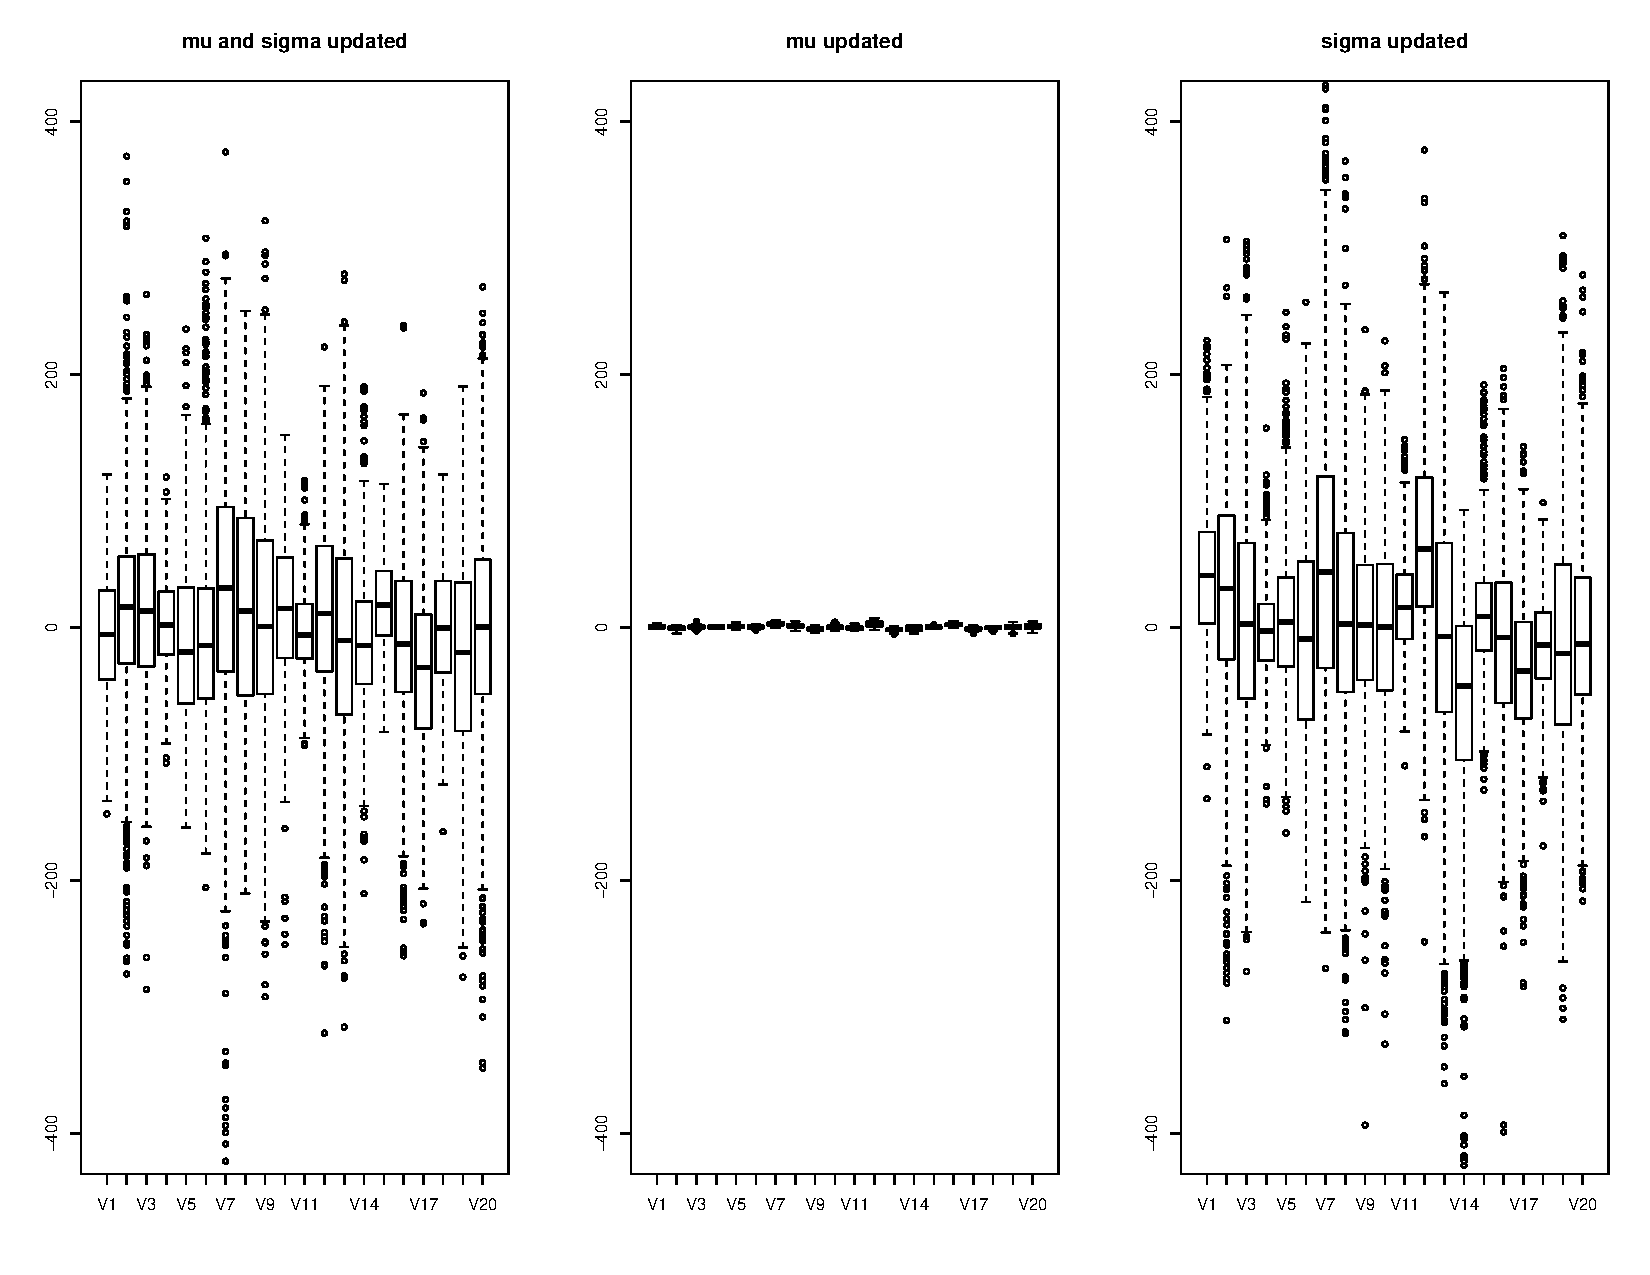
\includegraphics[width=14cm]{Boxplot_question_1.pdf}
\caption{Weight stability for a sub-sample of 500 days}
\label{fig1}
\end{figure}

As a result, we understand that weight instability and variability is primarily due to the estimation of $\Sigma$.
\par\smallskip
We conclude that we need a good estimation of the covariance matrix in order to calculate stable weights for our optimal portfolio. In our example we needed at least a sample size of 500 to get an invertible covariance matrix for 452 stocks, but this sample size is not sufficient to compute stable weights.  
 
